\chapter{Diagramas de estados (FSM)}
\label{ch:anexo_fsm}

Este anexo recoge los diagramas de estados completos de las máquinas de estados finitas (\ac{FSM}) más voluminosas del diseño, referenciadas desde sus respectivos módulos en el Capítulo~\ref{chap:desarrollo}. Se han trasladado aquí, en lugar de incluirse en el cuerpo del documento, debido a su tamaño.

% -----------------------------------------------------------------
\section{FSM de configuración del TOP}
\label{sec:anexo_fsm_top}

Diagrama de estados de la FSM principal \texttt{p\_fsm} (\texttt{TOP.vhd}), descrita textualmente en la Sección~\ref{sec:top}.

\begin{figure}[htbp]
    \centering
    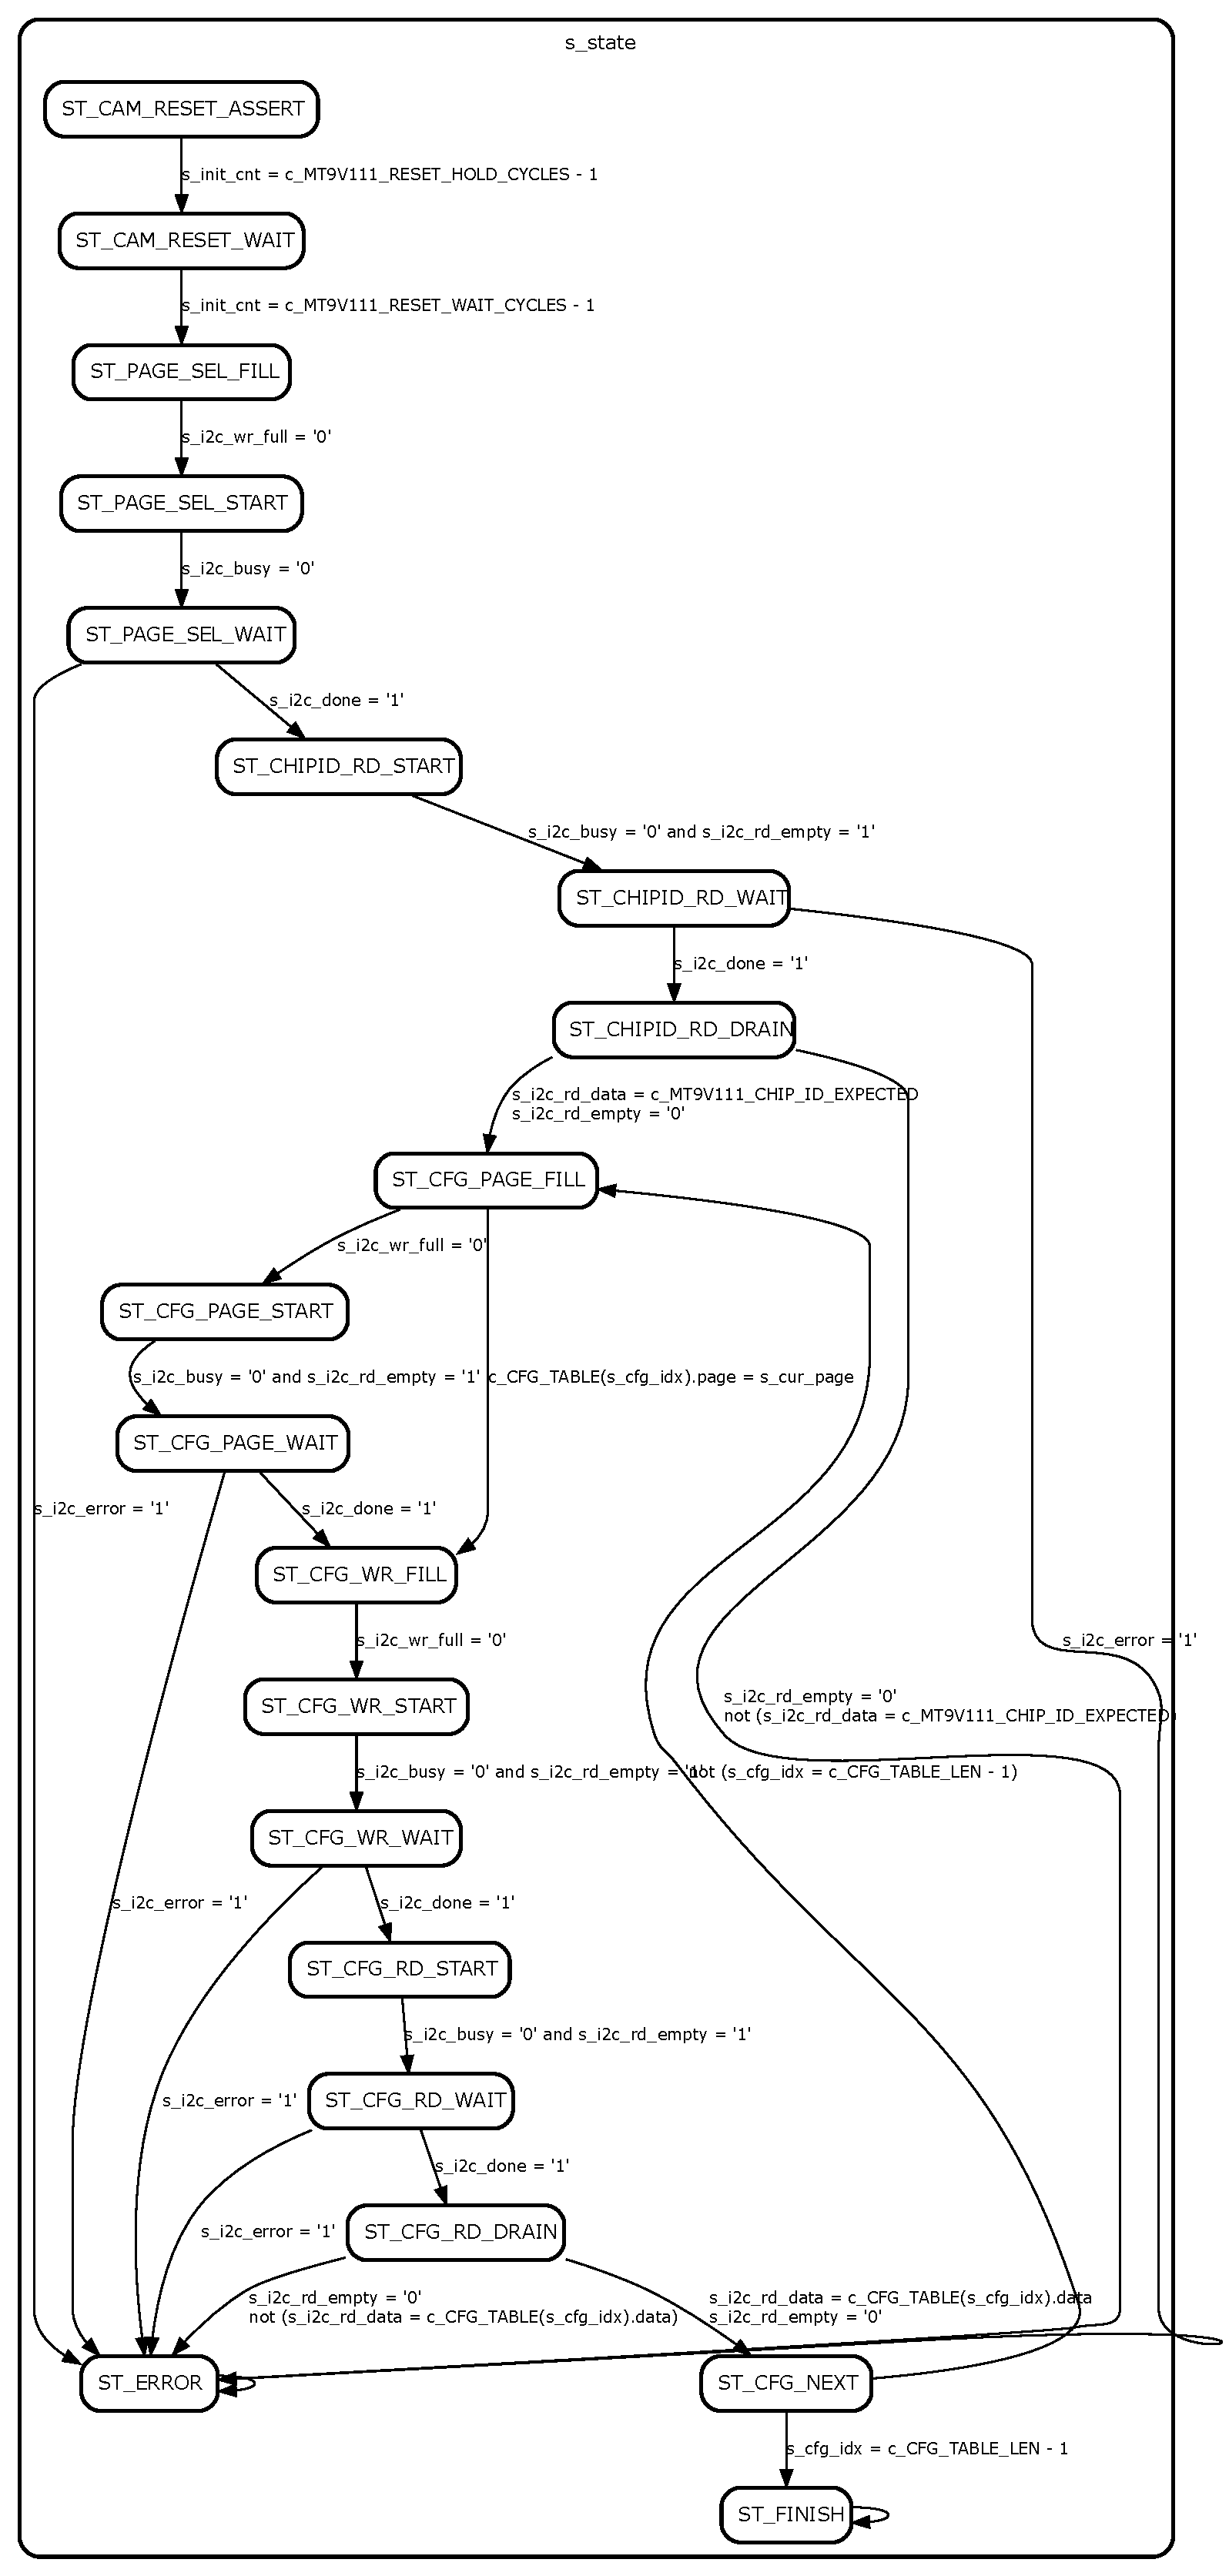
\includegraphics[width=0.7\textwidth]{gfx/anexo_fsm/fsm_top.pdf}
    \caption{FSM de configuración del sensor en \texttt{TOP.vhd}.}
    \label{fig:fsm_top}
\end{figure}

% -----------------------------------------------------------------
\section{FSM del \texttt{i2c\_controller}}
\label{sec:anexo_fsm_i2c}

Diagrama de estados completo del maestro \ac{I2C} \texttt{i2c\_controller.vhd} (37~estados, Tabla~\ref{tab:i2c_fsm}, Sección~\ref{sec:i2c_controller}).

\begin{figure}[htbp]
    \centering
    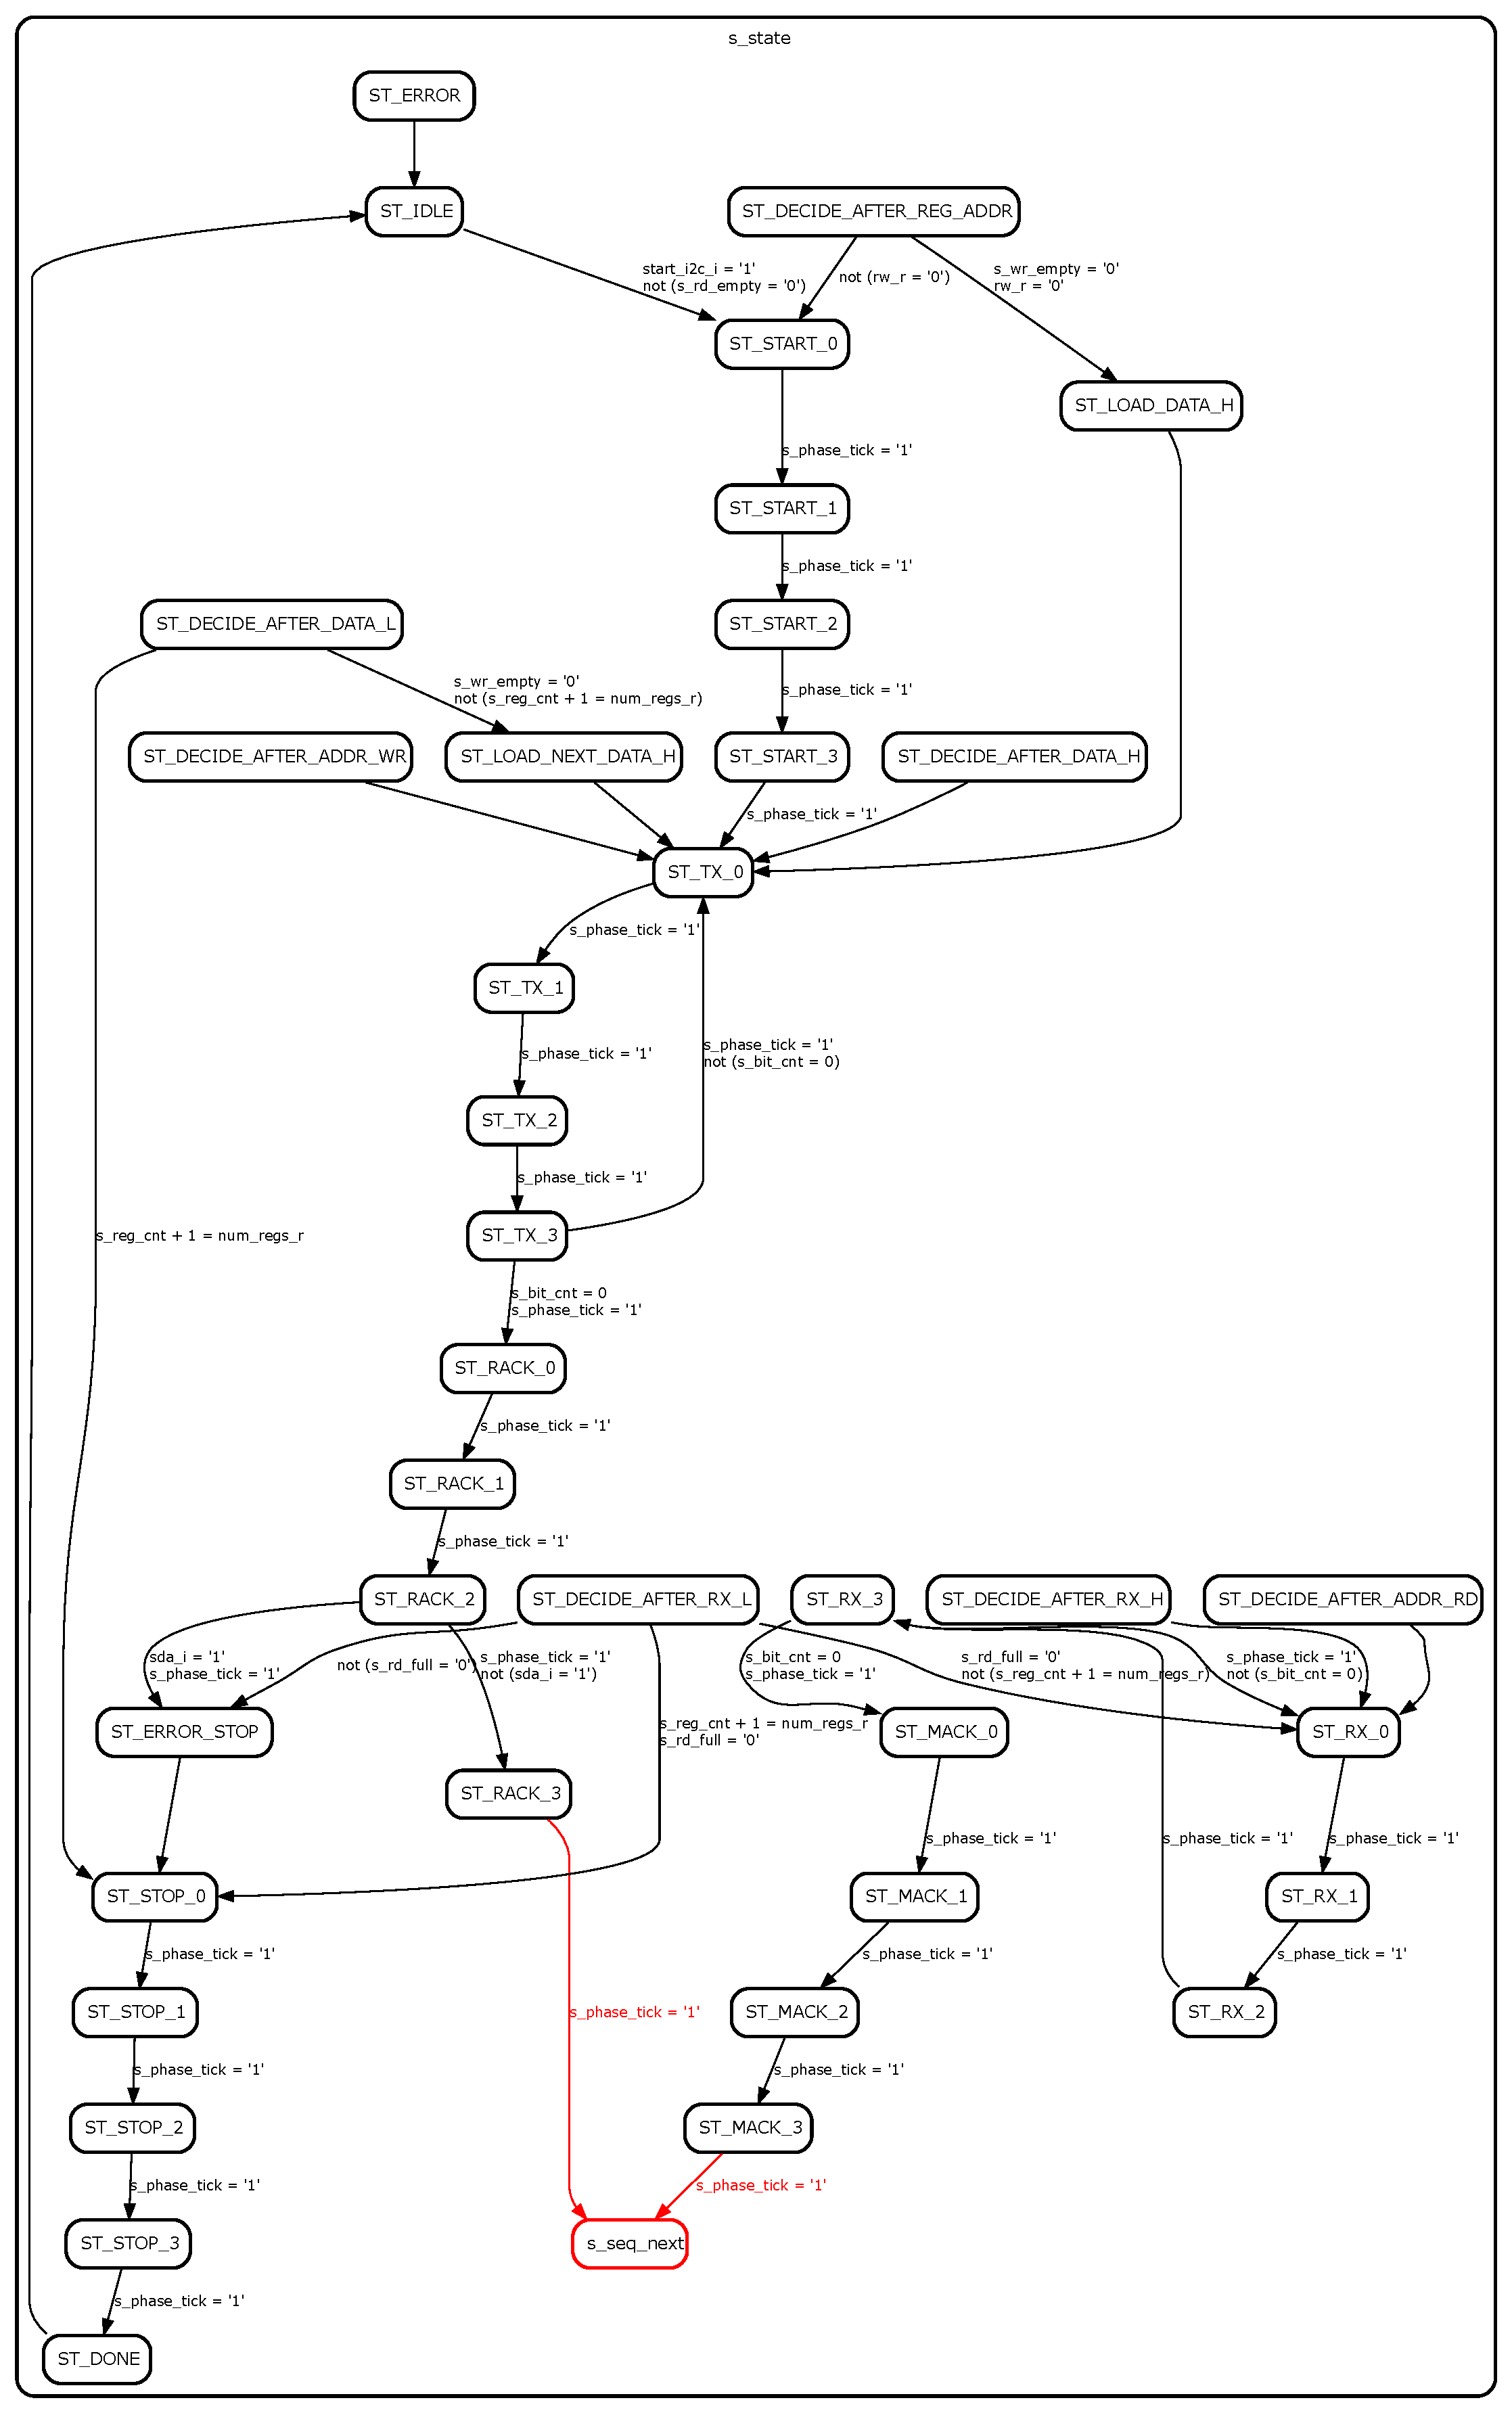
\includegraphics[width=0.7\textwidth]{gfx/anexo_fsm/fsm_i2c.pdf}
    \caption{FSM de \texttt{i2c\_controller.vhd}.}
    \label{fig:fsm_i2c}
\end{figure}

% -----------------------------------------------------------------
\section{FSM de recepción del \texttt{ftdi\_controller}}
\label{sec:anexo_fsm_ftdi}

Diagrama de estados del proceso \texttt{p\_rx} de \texttt{ftdi\_controller.vhd} (Sección~\ref{sec:ftdi_controller}), que gestiona la recepción de comandos PC$\rightarrow$FPGA en modo ráfaga continua.

\begin{figure}[htbp]
    \centering
    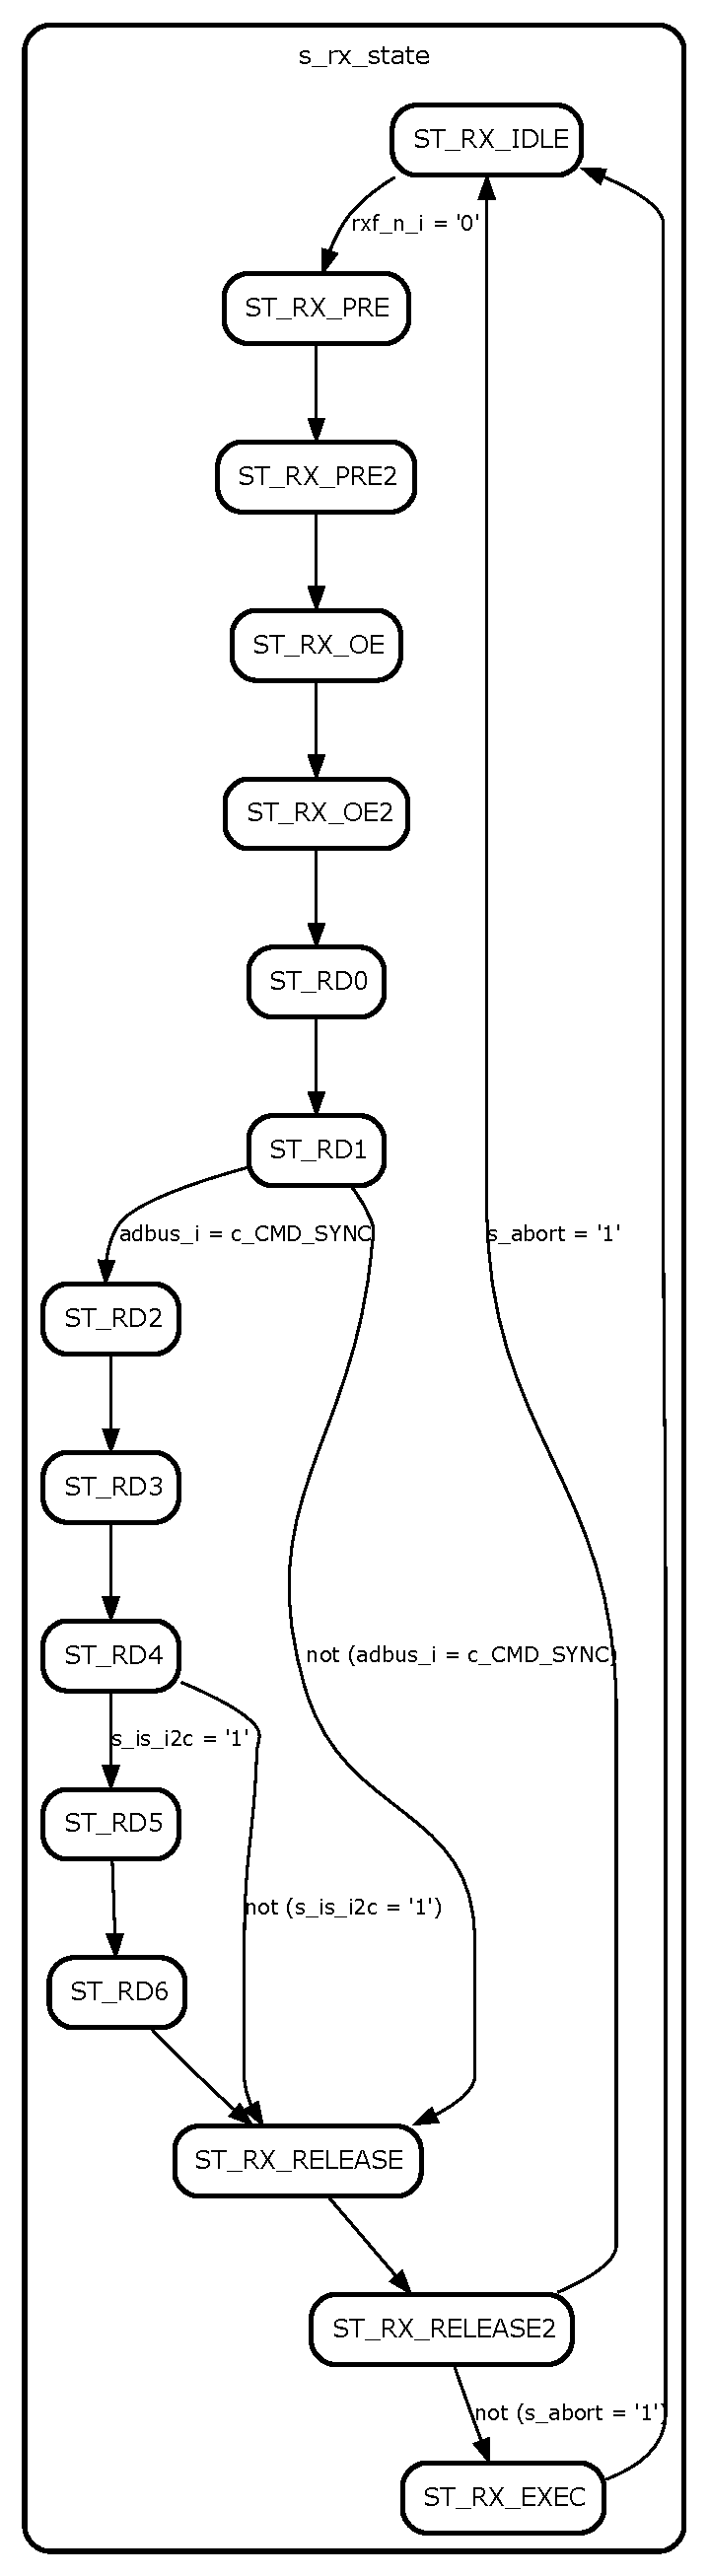
\includegraphics[width=0.35\textwidth]{gfx/anexo_fsm/fsm_ftdi.pdf}
    \caption{FSM de recepción (\texttt{p\_rx}) de \texttt{ftdi\_controller.vhd}.}
    \label{fig:fsm_ftdi_rx}
\end{figure}
